\documentclass[12pt]{book}

\usepackage{amsfonts,amsmath,amssymb}
\usepackage{graphicx}
\usepackage{color}
\usepackage{color,soul}
\usepackage[colorlinks,linkcolor=blue,citecolor=blue,urlcolor=blue,pdftitle={Balrog},pdfauthor={Suchyta}]{hyperref}
\usepackage[margin=1.0in]{geometry}
\usepackage{longtable}
\usepackage{tabu}
\usepackage{array}
\usepackage[singlelinecheck=false]{caption}

\usepackage{title}
\usepackage{optstable}
\usepackage{config}
\usepackage{outtable}
\usepackage{todonotes}

\renewcommand*\sectionautorefname{Section}
\renewcommand*\subsectionautorefname{Section}
\renewcommand*\subsubsectionautorefname{Section}

\newcommand{\py}{Python}
\newcommand{\balrog}{\textsc{Balrog}}
\newcommand{\sex}{\textsc{SExtractor}}
\newcommand{\psfex}{\textsc{PSFEx}}
\newcommand{\opt}[1]{\texttt{--#1}}
\newcommand{\inline}{\\[0.4cm]}
\newcommand{\bcmd}[1]{\texttt{\% runbalrog #1}}
\newcommand{\sersic}{S\'{e}rsic}

\newcommand\note[3]{\todo[color=#1, inline, size=\small]{#2: #3}}
\newcommand\notesuchyta[1]{\note{red!50}{EDS}{#1}}

\begin{document}
{\balrogtitlepage \let\cleardoublepage\clearpage \tableofcontents}

\chapter{What is \balrog{} and what is it good for?}
\section{Introduction}
\label{sec:intro}
\balrog{} is ...

\section{The \balrog{} Algorithm}
\label{sec:algorithm}

\balrog{} does ...

\begin{figure}[bh]
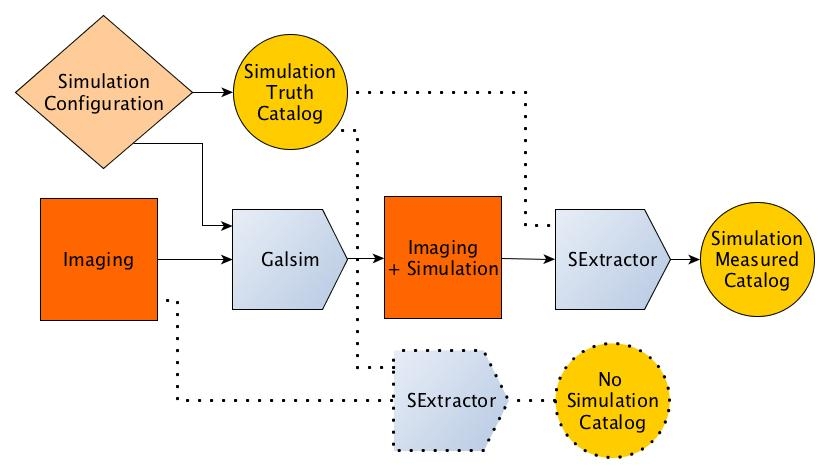
\includegraphics[width=0.9\linewidth]{flowchart.jpg}
\caption{Visualization of \balrog{}'s data flow. Optional configurations are represented as dotted connections.}
\label{fig:flowchart}
\end{figure}

\subsection{Postage Stamp Size}
\label{sec:postagestamp}

To get the postage stamps ...


\section{Science Motivation}
\label{sec:motivation}

What is \balrog{} good for?


\chapter{Installation}

\section{Installation}
\label{sec:install}

Installation is a bitch. Let your system administrator worry about it. 
But if you have to do it, here are some steps that \emph{might} work...

\begin{table}
\caption{Definitions used throughout this manual.}
\label{tab:def}
\begin{tabular}{l l}
\underline{\textbf{Name}} & \underline{\textbf{Meaning}} \\
\texttt{\$INSTALLDIR} & Directory where \balrog{} was installed \\
\texttt{runbalrog} & \texttt{\$INSTALLDIR/balrog.py} \\
\texttt{configfile} & \texttt{\$INSTALLDIR/config.py} \\
\multicolumn{2}{l}{\notesuchyta{I'm not sure where this table belongs, if it belongs anywhere at all.}}
\end{tabular}
\end{table}


\chapter{Quick Start}
\label{quick}

The fastest way to get started understanding how to configure and use \balrog{} is to
run it using the example files which come packaged with the software, and then examine the input
and output of the run. 
\balrog{} has been set up such that when the executable \py{}
file is called without any command line arguments, it will run over
the example files, filling in defaults as necessary. 
Thus, this inital call is as simple as:
\inline
\bcmd{}
\inline
Referring to \autoref{tab:def}, \texttt{runbalrog} is equivalent to an alias to the file
\texttt{balrog.py} located within the installation directory, labelled like an environment variable as \texttt{\$INSTALLDIR}. We will use these conventions
throughout the documentation. \autoref{sec:input} briefly addresses
the input which was read in for the \texttt{runbalrog} command and \autoref{sec:output} introduces the output
generated during the run.  \notesuchyta{Add text to see relevant later sections for more comprehensive details. For now I'm not quite sure what those are.}

\section{Input}
\label{sec:input}

\balrog{}'s input comes in two forms, command line arguments and \py{} statements.
The command line arguments can be printed, along with brief help string by running:
\inline
\bcmd{help}
\inline
Furthermore, a complete description of \balrog{}'s command line arguments can be found in \autoref{sec:cmdline}.
In brief, the command line parameters are used to specify input images and their properties, as well as configuration
files to use with \sex{}. The default example's image data and PSF live in \texttt{\$INSTALLDIR/default\_example/}.
The default \sex{} configuration files live in \texttt{\$INSTALLDIR/astro\_config}. File names are intended to be transparent.

In order to define how galaxies will be simulated, \balrog{} accepts defined blocks of code
within \texttt{configfile}. Included is support for implementing custom user-defined functions and command line arguments.
The default location for \balrog{} to look for this configuration file is noted in \autoref{tab:def}, within
the installation directory as a file named \texttt{config.py}. The core functions inside \texttt{configfile} have a strictly
defined syntax which will be fully described in \autoref{sec:cmdline} and \autoref{sec:simrules}. The syntax is designed to be as \py esque as possible, so
many users will likely be able to extrapolate directly from the examples in the default \texttt{configfile}. Additionally, the file
includes comments as a guide. A slightly more sophisticated \texttt{configfile} can be found in \texttt{\$INSTALLDIR/config2.py}.
The command line option \opt{config} is used to switch the file \balrog{} reads its configuration from.


\section{Output}
\label{sec:output}

All \balrog{} output is saved in subdirectories under the command line option \opt{outdir}.
If left unspecified, this defaults to \texttt{\$INSTALLDIR/default\_example/output}.
Most relevant for getting started are the \texttt{balrog\_cat} directory and the \texttt{balrog\_log} directory.
\texttt{balrog\_cat} contains \texttt{example.truthcat.sim.fits}, the truth parameters assigned to simulated galaxies
and \texttt{example.measuredcat.sim.fits}, the simulated galaxies properties as measured in the image by \sex{}.
\texttt{balrog\_log} saves log files useful for debugging \balrog{} runs.


\chapter{Detailed}
\section{Command Line Options}
\label{sec:cmdline}

\balrog{} runs can be configured via command line options.
Two types of options exist. First are the built-in
ones, native to \balrog{}. In addition, \balrog{}
supports a mechanism for users to define their
own command line options.
To print a list of all \balrog{}'s command line options,
both native and user-defined, along with
brief help strings, run:
\inline
\bcmd{\opt{help}}
\inline
\autoref{sec:builtin} further details each
of the native options and \autoref{sec:user}
explains how to create custom options.

\subsection{Built-in Options}
\label{sec:builtin}

\balrog{} includes a number of built-in optional arguments for each run, defining a
variety of parameters such as the input image,
the number of galaxies to simulate, the flux calibration, etc.
Any options which are not specified assume a default value.
The options are intended to be named intuitvely in order
to faciltate ease of use. 
\autoref{tab:opts} lists each option, with a description of 
what it means, including its default.
Abbreviations for each option also exist,
trading clarity for brevity.


\optstab{}

\subsection{User-defined Options}
\label{sec:user}

Within the \config{} file, user's are able to
define their own command line options. This occurs
within the function \argsfunc{}. Passed
to \argsfunc{}  as an argument is \argsparser{},
an object made by \texttt{python}'s
\texttt{argparse.ArgumentParser()}. Arguments
can be added to parser according to the usual
\texttt{argparse} syntax.
For those unfamilar with \texttt{argparse},
\href{http://docs.python.org/2/howto/argparse.html}{this tutorial}
contains many useful examples. A simple example of
\argsfunc{} is copied below.

\setlength{\tabcolsep}{0pt}
\begin{longtabu*} to \linewidth {l X}
\multicolumn{2}{l}{\texttt{def CustomArgs(parser):}}\\
\hspace{20pt} \texttt{parser.add\_argument(} & \texttt{"-cs", "--catalogsample", help="Catalog used to
sample simulated galaxy parameter distriubtions from", type=str, default=None)}
\end{longtabu*}
\setlength{\tabcolsep}{6pt}
\addtocounter{table}{-1}


User-defined options are parsed within the function \parsefunc{},
also part of \config{}.
Passed as an argument to \parsefunc{} is \parseargs{}, equivalent
to an object returned by \texttt{parser.parse\_args()}. Each one of the user's 
command line options becomes an attribute of \parseargs{}. 
A simple version of \parsefunc{} has been included below.

\setlength{\tabcolsep}{0pt}
\begin{longtabu*} to \linewidth {X}
\texttt{def CustomParseArgs(args):}\\
\hspace{20pt} \texttt{thisdir = os.path.dirname( os.path.realpath(\_\_file\_\_) )} \\
\hspace{20pt} \texttt{if args.catalogsample==None:} \\
\hspace{40pt} \texttt{args.catalogsample = os.path.join(thisdir, 'cosmos.fits')}
\end{longtabu*}
\setlength{\tabcolsep}{6pt}
\addtocounter{table}{-1}

\noindent The ability to define and parse one's own command line arguments is intended to make
\balrog{} flexible to conveniently running a wide variety of different
simulation scenarios. These parameters are available to the user 
when setting up the galaxy simulations. How to define these simulations is described in
\autoref{sec:simrules} below.

\section{Defining How to Simulate Galaxies}
\label{sec:simrules}

Defining how galaxies should be simulated is controlled within \config{}
in the function \simfunc{}. Passed into the function are three
arguments: \simargs{}, \simrules{}, and \simsamp{}.
\simargs{} refers to the parsed command line arguments,
both native \balrog{} and user-defined.
\simrules{} is an object whose components are overwritten
in order to specify how simulated galaxies are sampled.
\simsamp{} gives access to simulated galaxy parameters
after they have been sampled. \simrules{} and \simsamp{}
will become clearer to follow.

\balrog{} simulates galaxies as $N$ component \sersic{} profiles, 
where $N$ ranges from 1 to as many as desired. Associated
with each of these components are five attributes: a \sersic{} index,
half light radius, magnitude, axis ratio ($b/a$), and orientation
angle ($\beta$). In addition, each simulated galaxy has five attributes
common among each \sersic{} profile: $x$ and $y$-coordinates,
two components of reduced shear ($g_1$, $g_2$), and magnification.
\simfunc{}'s argument \simrules{} is comprised of attributes
for these different galaxy characteristics. Users overwrite
each of \simrules{}'s attributes to define their simulations.
For example the statement to set each galaxy's magnification
to 1 would read:
\inline
\texttt{magnification = 1}
\inline
\simrules{} has 11 attributes in total, whose names are intended to be simple to understand.
These are printed and desribed in \autoref{tab:attr} below.

\vspace{10pt}
\begin{longtabu} to \linewidth {l l}
\caption{Attributes of the rules defining the simulated galxies.} \label{tab:attr}\\
\underline{\textbf{Attribute}} & \underline{\textbf{Meaning}} \\
\texttt{rules.x} & Galaxy centroid $x$-coordinate [pixels], first pixel = 1\\
\texttt{rules.y} & Galaxy centroid $y$-coordinate [pixels], first pixel = 1\\
\texttt{rules.g1} & Reduced shear, $g_1$ component \\
\texttt{rules.g2} & Reduded shear, $g_2$ component \\
\texttt{rules.magnification} & Magnification, $1 + \kappa$ \\
\texttt{rules.nProfiles} & Number of superimposed \sersic{} profiles \\
\texttt{rules.sersicindex} & \sersic{} index \\
\texttt{rules.halflightradus} & \sersic{} half light radius \\
\texttt{rules.magnitude} & Galaxy brightness in magnitudes \\
\texttt{rules.axisratio} & Minor to major axis ratio, $b/a$ \\
\texttt{rules.beta} & Orientaiton angle of major axis (measured from $x$-axis)
\end{longtabu}

\noindent \texttt{rules.sersicindex}, \texttt{rules.halflightradius}, \texttt{rules.magnitude}, \texttt{rules.axisratio},
and \texttt{rules.beta} must be arrays, whose length is equal to \texttt{rules.nProfiles}. For example, simulating
galaxies with both an expontential and a de Vaucouleurs component would read:
\inline
\texttt{rules.nProfiles} = 2 \\
\texttt{rules.sersicindex = [1,4]}

Simulation rules can assume four types. The first is a constant, meaning each of the 
galaxies in the simulated galaxy sample
will have the same value for the selected parameter. 
Rules can also be assigned as an array, equal in length to the number of simulated galaxies. 
Simulated galaxy $i$ for the chosen parameter then assumes the value in element $i$ of
the array.
Additionally, sampling can be drawn from a catlog. Multiple
parameters selected from the same data table are automatically jointly sampled.
Finally a function can be used. Users write their own \texttt{python} function,
then feed this function and its necessary arguments as the arguments to
\balrog{}'s \texttt{Function} command. The defined function must return an
array equal in length to the number of simulated galaxies. Like the array
sampling type, galaxy $i$ will use element $i$ of the returned array.
Currently only positional arguments are supported within the user-defined
functions, but support for keyword arguments will be added.
\texttt{Function} affords both flexiblity and convenience when deciding
how to sample the simulated galaxies. See \config{} for examples
using \texttt{Function} as well as other sampling types.
One simple example of how to implement each of the four different 
types is shown in \autoref{tab:simtype}.

\vspace{10pt}
\setlength{\tabcolsep}{0pt}
\begin{longtabu} to \linewidth {p{1in} l X}
\caption{Syntax examples for each of the simulation types \balrog{} understands.} \label{tab:simtype} \\
\underline{\textbf{Type}} & \multicolumn{2}{l}{\underline{\textbf{Example}}} \\
Constant & \multicolumn{2}{l}{\texttt{rules.g1 = 0}} \\
Array & \texttt{rules.axisratio = [} & \texttt{np.ones(args.ngal)/np.arange(1,args.ngal+1), sampled.axisratio[0]]} \\
Catalog & \texttt{rules.magnitude = [} & \texttt{Catalog(`cosmos.fits', 0, `IMAG'), Catalog(`cosmos.fits', 0, `IMAG')]} \\
Function & \multicolumn{2}{l}{\texttt{rules.g2 = Function(function=NFW2, args=(sampled.x,sampled.y))}}
\end{longtabu}
\setlength{\tabcolsep}{6pt}

The second and fourth examples in \autoref{tab:simtype} makes use of \simsamp{}, the third argument
passed to \simfunc{}. \simsamp{} is an object allowing users to refer to the properties of
the simulated galaxies after they have been sampled. Referring to the second example above,
the first element of \texttt{rules.axisratio} is an array decreasing incrementally from 1 to 0.
The second elemment of \texttt{rules.axisratio} then says to use whatever the sampled values of
 the first element turn out to be. Here, this equates to setting the second element of \texttt{rules.axisratio}
 to the same array as the first element of \texttt{rules.axisratio}, so the use of \simsamp{} is not 
 really necessary. However, return to the fourth example in \autoref{tab:simtype}. Image \texttt{NFW2}
 as a function which takes two arguments, \texttt{x} and \texttt{y}, which returns the $g_2$ component
 of shear at position ($x$,$y$) from an NFW halo with mass $10^{15} M_{\odot}$ whose center lies at (0,0).
 Now image \texttt{sampled.x} and \texttt{sampled.y} were sampled randomly:
 
 \setlength{\tabcolsep}{0pt}
\begin{longtabu} to \linewidth {X}
\texttt{def Random(minimum, maximum, size):} \\
\hspace{20pt}  \texttt{return np.random.uniform(minimum, maximum, size)}\\
\\
\texttt{rules.x = Random(args.xmin, args.xmax, args.ngal)} \\
\texttt{rules.y = Random(args.ymin, args.ymax, args.ngal)}
\end{longtabu}
\setlength{\tabcolsep}{6pt}
\addtocounter{table}{-1}
 
\noindent \texttt{sampled.x} and \texttt{sampled.y} now represent the values
for $x$ and $y$ after the random sampling has occurred. 
Along these lines, \balrog{} can build-up simulations with fairly little recoding between completely
different types of simulations.
\balrog{} makes sure that all the simulation parameters are sampled
in the proper order and will throw an error if something ambiguous was defined
by the user.


\section{Output}
Each \balrog{} run generates a number of output files. 
These are organized into a fixed directory structure.
Users indicate the \opt{outdir} command line option, and
the remainder of the naming scheme occurs automatically,
placing files in subdirectories under \opt{outdir}.
Four subdirectories are written, labelled accoring to what
type of files they contain. \autoref{tab:out}
lists the contents of each of these subdirectories,
giving a brief desription of each file. Depending on how
\balrog{} was configured, not necessarily every file
in \autoref{tab:out} will be present in every run.
The \texttt{*} symbol in \autoref{tab:out} will be replaced with
the base name of the input image file. For example,
if the input image is named \texttt{example.fits},
\texttt{*} will be replaced with \texttt{example}.
If the input file name does not end with the \texttt{.fits}
extension, the file name itself is used as the base name.
This does not include any diretories preceeding the file name.
For example, if the input image was given as
\texttt{/Users/somebody/home/image.f}, the
base name would be \texttt{image}.

\outtab{}

\section{Debugging}
\label{sec:debug}


\end{document}
